\documentclass[tikz,border=2mm]{standalone}
\usepackage{tikz}
\usetikzlibrary{shapes.geometric, arrows, shapes.gates.logic.US, calc}

\tikzstyle{arrow} = [thick,->,>=stealth]

\begin{document}
    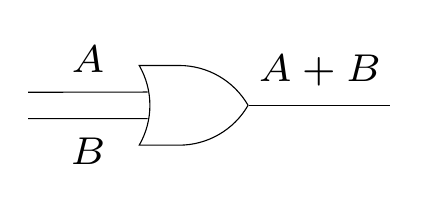
\begin{tikzpicture}[node distance=2cm, scale=2, every node/.style={scale=2}]
        
        \node at (1,-0.25) [or gate US, logic gate inputs=nn,draw](and) {};
        
        \draw (and.output) -- node[above]{\scriptsize $A + B$} (2.3, -0.25);
        \draw (0,-0.167) -- node[above]{\scriptsize $A$} (and.input 1);
        \draw (0,-0.334) -- node[below]{\scriptsize $B$} (and.input 2);
        
    \end{tikzpicture}
\end{document}
